\chapter{Science in the Community}

\begin{multicols}{2}


\section{Science for All}

\begin{center}
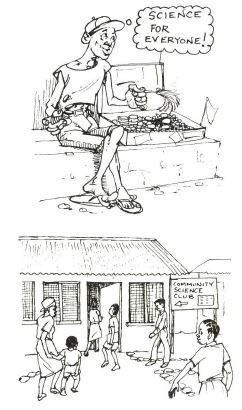
\includegraphics[width=0.45\textwidth]{./img/source/science-for-all.jpg}
\end{center}

Science clubs and activities are most often school based,
but they may be organised at a science centre,
community hall, factory or business.
In many countries a large proportion of the
school age populations are not at school, and
never will be. They receive only the barest
contact during elementary years and thus may
have no real opportunity to learn or experience
science and technology. 

Therefore, the potential
for out-of-school science and technology
education is enormous, ranging from the vast
numbers of adults to the large numbers of school-age
leavers who have had no formal education
or inadequate contact with science education.

How can your school and community help
spread and share science for all?
A community science club may be the answer - a
joint venture between school and community.


\section{Science Target Groups}

\begin{center}
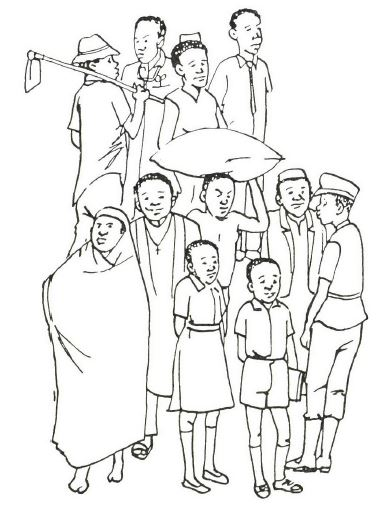
\includegraphics[width=0.45\textwidth]{./img/source/target-groups.jpg}
\end{center}

``A1l out-of-school science activities and.
programmes should be planned and developed
according to the identified needs, interests
real-life problems and concerns of the various
target groups.'' (UNESCO)

(a) The formal school populations, who need
out-of-school activities to enrich, supplement
and complement school science education
curricula.

(b) Out of school youth and adults (early
dropouts from school, illiterates, general work
force), who need activities designed to develop
a basic scientific literacy, to create interest and
to form an appropriate, relevant scientific
climate of opinion.

(c) Educated youths and adults for whom out-of-school activities should be part of a lifelong
education, designed to clarify changing socioeconomic
and cultural conditions and rapid
changes in the applications and relevance of
scientific and technological ideas and
developments.


\section{Environmental \hfill \\ Awareness}

\begin{center}
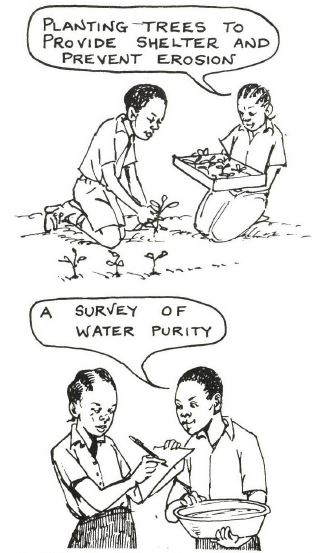
\includegraphics[width=0.45\textwidth]{./img/source/environmental-awareness.jpg}
\end{center}

A vital role of a science club or group is to raise
environmental awareness in the school and
community. Millions of people are very
concerned about what is happening to our world
and looking for ways to change things for the
better. Perhaps you think that means you don't
have to get involved, or that the environment is
getting enough attention. Nothing could be
further from the truth - the battle is nowhere near
won! 

This can take the form of surveys, plays,
studies, posters, discussions and debates. Many
socially beneficial environmental protection
activities can be undertaken, such as the creation
of specific mini-nature reserves or patches, tree
and shrub planting to prevent erosion and provide
shade; protecting newly planted trees from
animals; beautifying ones home and greening of
street and courtyards. 

One of the most important
roles of the club in the community is to look-out
for environmental hazards like water pollution
which may affect everyone's health and
happiness.


\section{Wildlife Conservation}

\begin{center}

\includegraphics[width=0.45\textwidth]{./img/source/wildlife.jpg}
\end{center}

Out-of-school activities give an excellent
opportunity for students to collect and study
small wild creatures. The teacher must instruct
the students to be careful not to distress the
animals while the study is being carried out.

Wherever possible living things should be
studied in their own habitats. If this is not
possible and they have to be captured, the
students MUST try to return the animals to their
original home. Students must be made aware
that by destroying wildlife habitats they destroy
the wildlife. By protecting habitats Tanzania's
precious wildlife resources will be conserved
for future generations.


\section{Science and Health}
% ref HIV/AIDS, malaria, drug use in activities

\begin{center}
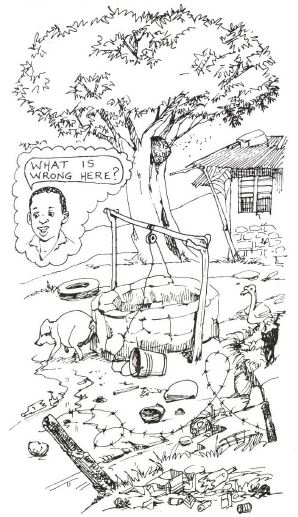
\includegraphics[width=0.45\textwidth]{./img/source/science-health.jpg}
\end{center}

Health education is part of school science,
but can also be a major focus for out-of-school
activities. Good science teaching and scientific
thinking can improve health. Health education
is concerned with skills for life: skills which can
save and improve lives; skills which go out of
the classroom and are used in daily life and
which, when thoroughly learnt, last for life.

Pollution of the environment is the major cause
of health problems in a community. Students
need to be able to identify polluting health
hazards in the local environment. Health is one
of the areas which confirms to students that
scientific thinking need not be confined to the
laboratory but should be applied in many
different situations.


\end{multicols}